\section{140 - K5 - AG 2.3 - Basketball - UrsAlb}

\begin{langesbeispiel} \item[4] %PUNKTE DES BEISPIELS
Beim Basketball wird ein Ball in den Korb geworfen. Die Flugbahn des Balles entspricht etwa dem Graphen der Funktion 
$f(x) = -0,5x^2 + 3x - 1,5$, wobei man auf der 1. Achse die Zeit (in s) und auf der 2. Achse die Höhe (in m) ablesen kann.

\begin{center}
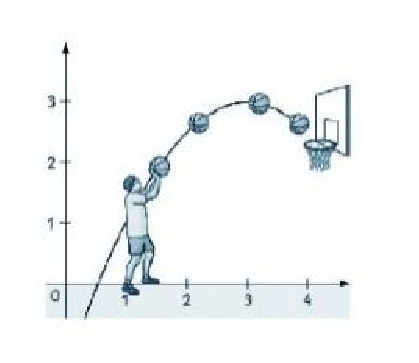
\includegraphics[width=0.4\textwidth]{../_database/Bilder/140_Basketball.eps}
\end{center}


Diese Funktion entspricht der  Gleichung $-0,5x^2+3x-1,5=0$, wenn der Ball am Boden liegt.%Aufgabentext

\begin{aufgabenstellung}
\item %Aufgabentext

\Subitem{Löse die quadratische Gleichung und runde deine Antworten auf zwei Dezimalstellen.} %Unterpunkt1
\Subitem{Wann erreicht das Spielgerät eine Höhe von 2 m?} %Unterpunkt2

\item %Aufgabentext

\Subitem{Erkläre, warum es die Höhe 2 m zwei Mal gibt?} %Unterpunkt1
\Subitem{Kreuze die beiden zutreffenden Aussagen an!\vspace{0,3cm}

\multiplechoice[5]{  %Anzahl der Antwortmoeglichkeiten, Standard: 5
				L1={Eine quadratische Gleichung hat mindestens zwei Lösungen in $\mathbb{R}$.},   %1. Antwortmoeglichkeit 
				L2={Eine quadratische Gleichung hat höchstens zwei Lösungen in $\mathbb{R}$ .},   %2. Antwortmoeglichkeit
				L3={Eine quadratische Gleichung kann nur zwei Lösungen $\mathbb{R}$ haben.},   %3. Antwortmoeglichkeit
				L4={Eine quadratische Gleichung hat mindestens eine Lösung in $\mathbb{R}$.},   %4. Antwortmoeglichkeit
				L5={Eine quadratische Gleichung kann keine Lösungen $\mathbb{R}$ haben.},	 %5. Antwortmoeglichkeit
				L6={},	 %6. Antwortmoeglichkeit
				L7={},	 %7. Antwortmoeglichkeit
				L8={},	 %8. Antwortmoeglichkeit
				L9={},	 %9. Antwortmoeglichkeit
				%% LOESUNG: %%
				A1=2,  % 1. Antwort
				A2=5,	 % 2. Antwort
				A3=0,  % 3. Antwort
				A4=0,  % 4. Antwort
				A5=0,  % 5. Antwort
				}} %Unterpunkt2

\end{aufgabenstellung}
\begin{loesung}
\item \subsection{Lösungserwartung:} 

\Subitem{$-0,5x^2+3x-1,5=0$, $\rightarrow x_1=1$ und $x_2=5$} %Lösung von Unterpunkt1
\Subitem{$-0,5x^2+3x-1,5=2$, $\rightarrow x_1  \approx 1,59$ und $x_2  \approx 4,41$} %%Lösung von Unterpunkt2

\setcounter{subitemcounter}{0}
\subsection{Lösungsschlüssel:}
 
\Subitem{Ein Punkt für die richtigen Lösungen.} %Lösungschlüssel von Unterpunkt1
\Subitem{Ein Punkt für die richtigen Lösungen.} %Lösungschlüssel von Unterpunkt2

\item \subsection{Lösungserwartung:} 

\Subitem{Da die Flugbahn parabelförmig ist, befindet sich der Körper einmal beim Flug hinauf und einmal beim Flug hinunter auf dieser Höhe.} %Lösung von Unterpunkt1
\Subitem{MC: siehe oben} %%Lösung von Unterpunkt2

\setcounter{subitemcounter}{0}
\subsection{Lösungsschlüssel:}
 
\Subitem{Ein Punkt für die richtige Interpretation.} %Lösungschlüssel von Unterpunkt1
\Subitem{Ein Punkt für die richtigen Lösungen.} %Lösungschlüssel von Unterpunkt2

\end{loesung}

\end{langesbeispiel}